\usepackage{bm} % To put math text in bold
\usepackage{hyperref}

%\usetheme{vub}
\usetheme[coloredtitles]{vub}
%\usetheme[showsection]{vub}

\title{Knowledge transfer in deep reinforcement learning}
% \subtitle{Master thesis}
\author{Arno Moonens}
\date{June 30, 2017}

% To center the contents of a frame vertically
\makeatletter
\define@key{beamerframe}{c}[true]{% centered
  \beamer@frametopskip=0pt plus 1fill\relax%
  \beamer@framebottomskip=0pt plus 1fill\relax%
  \beamer@frametopskipautobreak=0pt plus .4\paperheight\relax%
  \beamer@framebottomskipautobreak=0pt plus .6\paperheight\relax%
  \def\beamer@initfirstlineunskip{}%
}
\makeatother

% To change footnote size
\let\oldfootnotesize\footnotesize
\renewcommand*{\footnotesize}{\oldfootnotesize\tiny}

\setbeamertemplate{caption}{\raggedright\insertcaption\par}

\AtBeginPart{\frame{\partpage}}
% \AtBeginSection{\frame{\sectionpage}}
% \AtBeginSubsection{\frame{\subsectionpage}}

\graphicspath{ {../images/} }

\makeatletter
\def\beamer@framenotesbegin{% at beginning of slide
  \gdef\beamer@noteitems{}%
  \gdef\beamer@notes{{}}% used to be totally empty.
}
\makeatother

\begin{document}
\frame{\titlepage}

\begin{frame}{Outline}
    \vskip0pt plus 3fill
  {\color{vubbleu}\large Background}
  \tableofcontents[part=1]

  {\color{vubbleu}\large Experiments}
  \tableofcontents[part=2]

  {\color{vubbleu}\large Conclusions}
  \tableofcontents[part=3]
  \note{
  \begin{itemize}
      \item Goal: algorithm that is combination of deep RL algorithm and transfer learning
      \item First: discuss necessary knowledge
  \end{itemize}
  }
\end{frame}

\part{Background}

\section{Artificial neural networks}
\begin{frame}[fragile]\frametitle{Artificial neural networks}
% \framesubtitle{Architecture}
\vskip0pt plus 3fill
\begin{columns}
\begin{column}{0.5\textwidth}
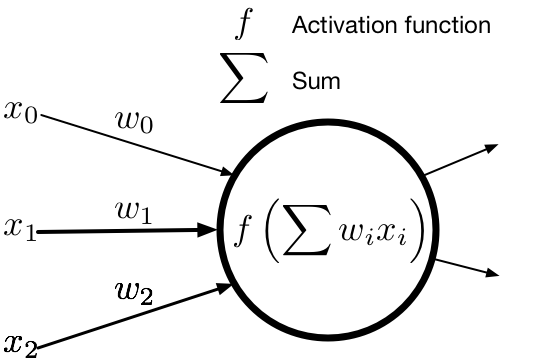
\includegraphics[width=\linewidth]{neuron.png}
\end{column}
\vrule
\begin{column}{0.5\textwidth}
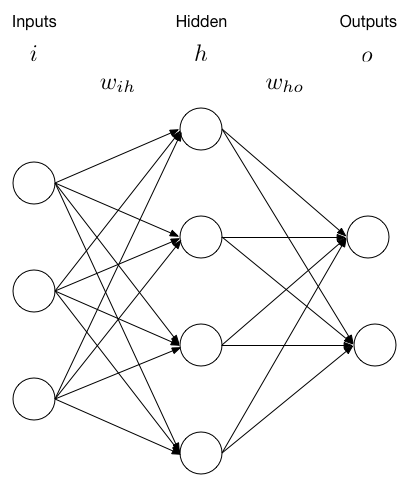
\includegraphics[width=\linewidth]{ann.png}
\end{column}
\end{columns}
\note{
    \begin{itemize}
        \item ANN = function approximator
        \item multiple layers each with units
        \begin{itemize}
            \item Input layer: its values is the data
            \item (Hidden layer(s)): Both receive info of units and get used by units of other layers
            \item Output layer: uses inputs of previous layer, output is directly
        \end{itemize}
        \item each unit: non-linear function of linear combination of units at previous layer
        \item each connection between units can vary in strength
        \item Error is differentiated to compute change in weights (backpropagation)
    \end{itemize}
}
\end{frame}

\section{Deep learning}
\begin{frame}[t]\frametitle{Deep learning}
\framesubtitle{Convolutional neural networks}
\vskip0pt plus 0.9fill
\begin{center}
    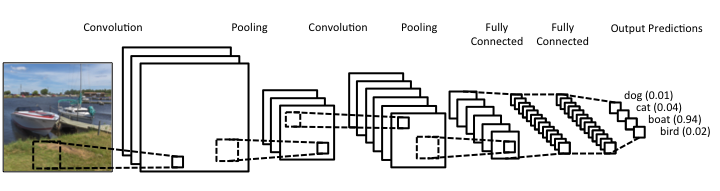
\includegraphics[width=\linewidth]{cnnlayout.png} \footnote{Source: \cite{clarifai}}\\
    \vskip0pt plus 0.1fill
    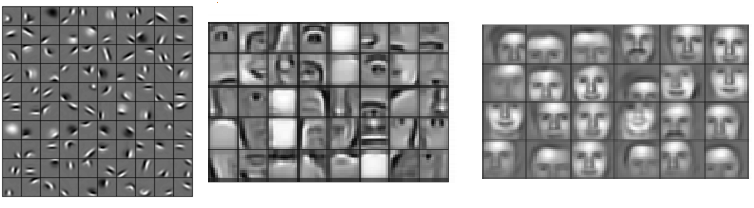
\includegraphics[width=\linewidth]{cnnfeatures.png} \footnote{Source: \cite{conf/icml/LeeGRN09}}
\end{center}
\note{
\begin{itemize}
    \item Handle high-dimensional data
    \item CNN = primarily used for images
    \item Filter is matrix of weights smaller than image
    \item Slide filter over image
    \item Only this filter is used instead of connection for every pixel
    \item Each level higher level representations
\end{itemize}
}
\end{frame}

\section{Reinforcement learning}
\begin{frame}[fragile]\frametitle{Reinforcement learning}
\vskip0pt plus 1fill
\begin{center}
    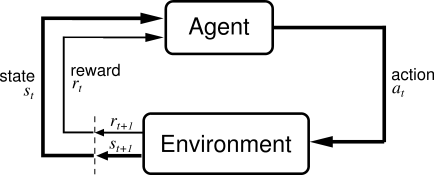
\includegraphics[width=.7\linewidth]{reinforcementlearning.png}
    \footnote{Source: \url{https://www.analyticsvidhya.com/blog/2017/01/introduction-to-reinforcement-learning-implementation/}}
\end{center}
\begin{itemize}
    \item Goal: maximize total reward
    \begin{itemize}
        \item By changing its policy $\pi$
    \end{itemize}
    \item Policy gradient:
    \begin{itemize}
        \item Policy is parametrized: $\pi_\theta(s,a)$
        \item Input: states
        \item Output: action (probabilities)
    \end{itemize}
\end{itemize}
\note{
    \begin{itemize}
        \item Learn by trial-and-error
        \item Do action in a state -> get reward
        \item Use policy to select actions
        \item Action produced using value function for state and action or directly: policy gradient
        \item Policy gradient:
        \begin{itemize}
            \item Parameterized policy
            \item Action probabilities
            \item Parameters updated to improve rewards
        \end{itemize}
    \end{itemize}
}
\end{frame}

\section{Deep reinforcement learning}
\begin{frame}[fragile]{Deep reinforcement learning}
\framesubtitle{A3C architecture}
\vskip0pt plus 10fill
\begin{center}
    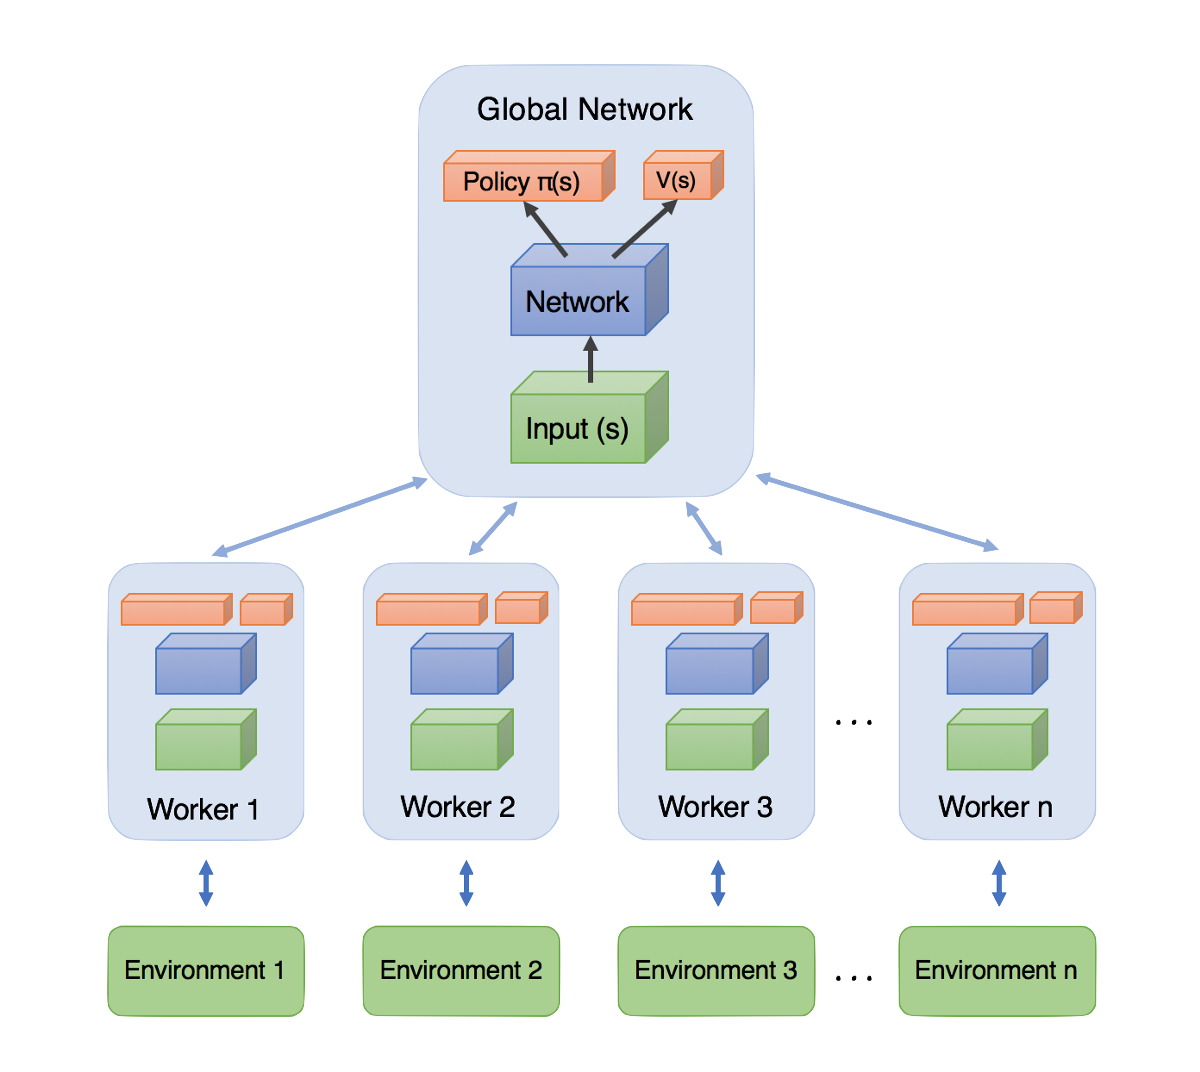
\includegraphics[width=.7\linewidth]{A3Carchitecture} \footnote{Source: \cite{Juliani2016A3C}}
\end{center}
\note{
    \begin{itemize}
        \item Combination of deep learning \& reinforcement learning
        \item Applied on environments with images as input
        \item Able to deal with correlated subsequent observations (they cause instability)
        \item A3C
        \begin{itemize}
            \item Learn in parallel on same kind of environment (same parameters)
            \item Global network with all the weights
            \item Each worker has copy
            \item Worker learns and then updates weights of global network
        \end{itemize}
    \end{itemize}
}
\end{frame}

\section{Transfer learning}
\begin{frame}[fragile]{Transfer learning}
\vskip0pt plus 1fill
\begin{columns}
\begin{column}{0.4\textwidth}
\begin{itemize}
    \item Which knowledge?
    \item From which tasks?
    \item How are tasks related?
    \begin{itemize}
        \item Same state space?
        \item Same action space?
    \end{itemize}
    \item Which RL algorithms are allowed?
\end{itemize}
\end{column}
    \begin{column}{0.6\textwidth}
    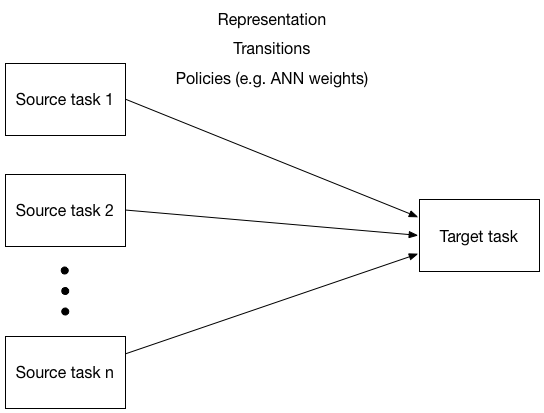
\includegraphics[width=\linewidth]{transfer_learning}
    \end{column}
\end{columns}
\begin{center}
\end{center}
\note{
    \begin{itemize}
        \item Use information about source task(s) to improve target task performance
        \item For example same game with different difficulty
        \item Improve:
        \begin{itemize}
            \item Jumpstart, Asymptotic, Total reward, Time until threshold
        \end{itemize}
        \item Transfer representation (FE), transitions or policies
        \item Tasks with same/different state and action space
        \begin{itemize}
            \item Task mapping may be necessary
            \item To use information about source tasks on target task
        \end{itemize}
    \end{itemize}
}
\end{frame}

\part{Experiments}
\section{Proposed algorithm}
\begin{frame}[fragile]{Proposed algorithm}
\framesubtitle{Architecture}
\vskip0pt plus 1fill
\begin{center}
    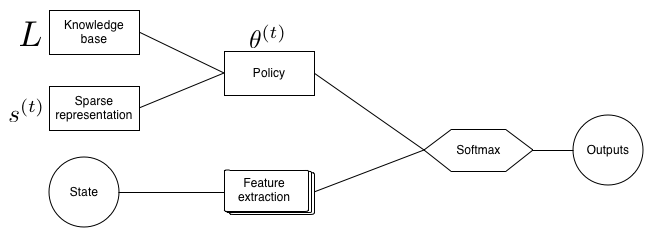
\includegraphics[width=\linewidth]{knowledge_transfer.png}
\end{center}
\note{
    \begin{itemize}
        \item combines transfer learning with A3C
        \item Architecture for a specific task $t$
        \item Uses policy gradient
        \item Policy factorized as knowledge base \& sparse representation
        \begin{itemize}
            \item Shared knowledge base: information common amongst tasks
            \item Shared feature extraction
            \item Each task has own sparse representation: how task differs from common knowledge
            \item Sparse repr actually kept sparse by adding value to error: L1 loss
        \end{itemize}
        \item Softmax to get action probabilities
    \end{itemize}
}
\end{frame}

\begin{frame}[fragile]{Proposed algorithm}
\framesubtitle{Learning source tasks}
\vskip1.5cm plus 2fill
\begin{center}
    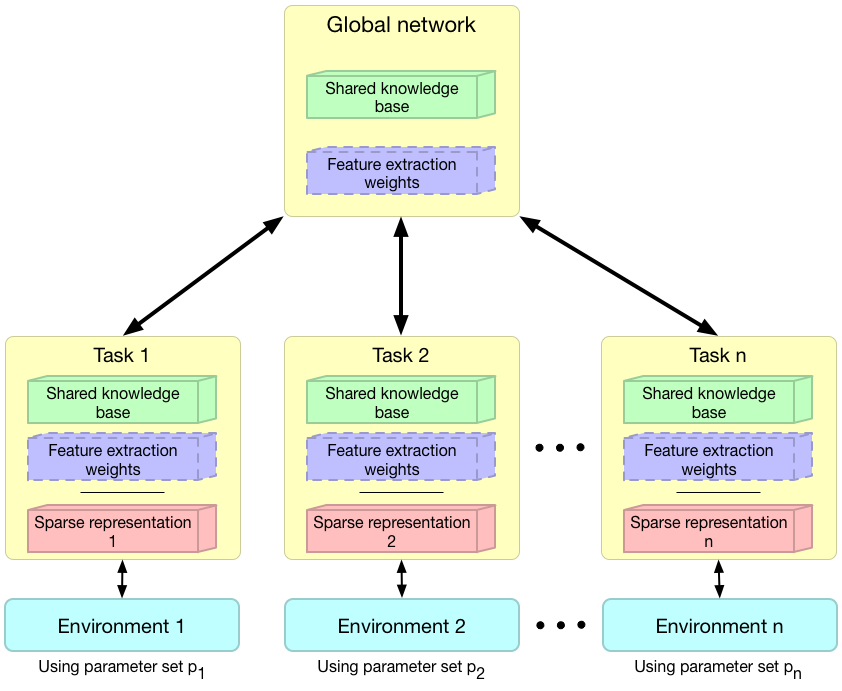
\includegraphics[width=.75\linewidth]{knowledge_transfer_tasks.png}
\end{center}
\note{
    \begin{itemize}
        \item Similar to A3C
        \item Global network has no sparse representation
        \item Each environment has different parameters (next slide)
        \item Source tasks learned sequentially or in parallel
        \item Global network is always transferred to target task
        \item Random sparse repr. can also be transferred
        \item On target task: only sparse repr can be changed!
    \end{itemize}
}
\end{frame}

\section{Experimental setup}
\begin{frame}[fragile]{Experimental setup}
\framesubtitle{Environments}
\vskip1.1cm plus 2.5fill
\begin{figure}[htb]
    \begin{minipage}{0.55\textwidth}
            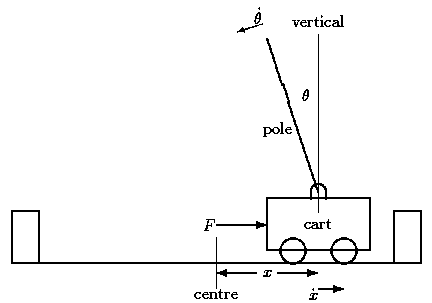
\includegraphics[width=\linewidth]{cartpole.png}
            \caption{Cart-pole \cite{grant1990modelling}.}
            \vskip0.9cm
            \begin{itemize}
                \item Different cart mass
                \item Different pole mass \& length
            \end{itemize}
    \end{minipage}\hfill
    \begin{minipage}{0.45\textwidth}
            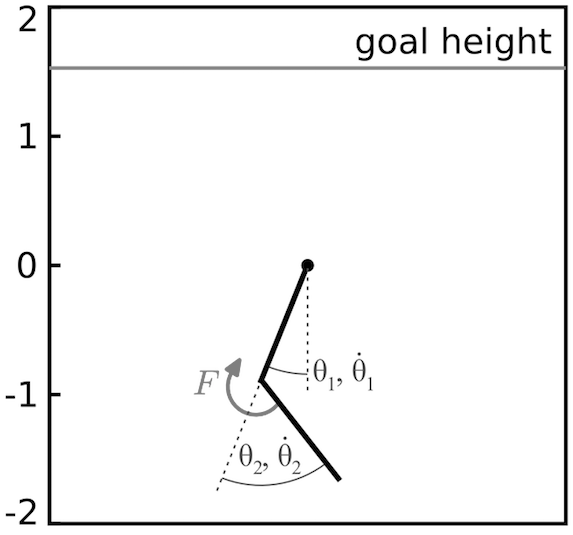
\includegraphics[width=\linewidth]{acrobot.png}
            \caption{Acrobot \cite{fremaux2013reinforcement}.}
            \begin{itemize}
                \item Different length \& mass for each pole
            \end{itemize}
    \end{minipage}
\end{figure}
\note{
    \begin{itemize}
        \item Cart-pole:
        \begin{itemize}
            \item Balance pole vertically on cart as long as possible
            \item Force on cart
            \item Different cart mass
            \item Different pole mass \& length
        \end{itemize}
        \item Acrobot:
        \begin{itemize}
            \item 2 joint arms
            \item Outer point must be above threshold in min. steps
            \item Different arm lengths and masses
        \end{itemize}
    \end{itemize}
}
\end{frame}

\section{Results}
\frame{\sectionpage}
\begin{frame}[fragile]{Parallel and sequential knowledge transfer}
\framesubtitle{Cart-pole}
\vskip0pt plus 3fill
\begin{center}
    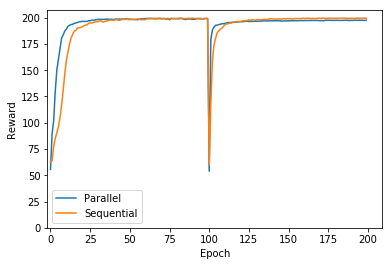
\includegraphics[width=.8\linewidth]{results/CartPole/kt_akt/reward_source-target_5tasks.png}
\end{center}
\note{
    \begin{itemize}
        \item Source tasks until epoch 100; then target task
        \item About the same asymptotic performance
        \item Parallel version is faster (higher total reward (Area Under Curve))
        \item Parallel: changes get applied immediately and effect other tasks
        \item Sequential: changes are accumulated and applied after evaluating every task
        \item Following experiments: parallel version
    \end{itemize}
}
\end{frame}

\begin{frame}[fragile]{Feature extraction}
\framesubtitle{Cart-pole}
\vskip0pt plus 3fill
Feature extraction layer with 5 and 10 units.
\begin{center}
    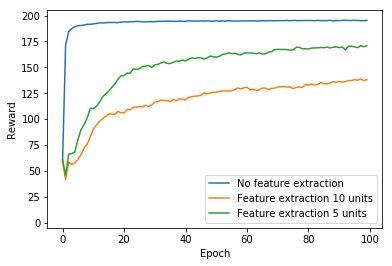
\includegraphics[width=.8\linewidth]{results/CartPole/feature_extraction.png}
\end{center}
\note{
    \begin{itemize}
        \item Feature extraction does not seem necessary
        \begin{itemize}
            \item It slows down learning
        \end{itemize}
        \item In general it's necessary for high-dimensional input spaces
        \item (there was no time to disassemble Atari games)
        \item Following experiments: no feature extraction
    \end{itemize}
}
\end{frame}

\begin{frame}[fragile]{Different amount of tasks}
\framesubtitle{Cart-pole}
\vskip1.5cm plus 0.5cm minus 0.1cm
Using 5 and 10 tasks, compared with \textit{REINFORCE}.
\begin{center}
    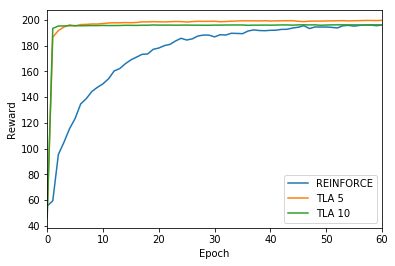
\includegraphics[width=.6\linewidth]{results/CartPole/no_sparse_transfer/reward_target_re-akt5-akt10.png}
\end{center}
\begin{tabular}{llccc}
\hline
Algorithm & Mean & Standard deviation & Median \\
\hline
   REINFORCE  & $86.060$ & $25.330$ & $86.886$ \\
   \textit{TLA 5} & $158.237$ & $23.153$ & $163.840$ \\
   \textit{TLA 10} & $\bm{165.120}$ & $21.955$ & $\bm{169.034}$ \\
\hline
\end{tabular}
\note{
    \begin{itemize}
        \item target task performance
        \item REINFORCE directly on target task
        \item Faster convergence than \textit{REINFORCE}
        \item Jumpstart TLA 10 > TLA 5 > REINFORCE
        \item Same asymptotic performances
    \end{itemize}
}
\end{frame}

\begin{frame}[fragile]{Different amount of source tasks}
\framesubtitle{Acrobot}
\vskip0pt plus 3fill
\begin{figure}[htb]
    \centering
    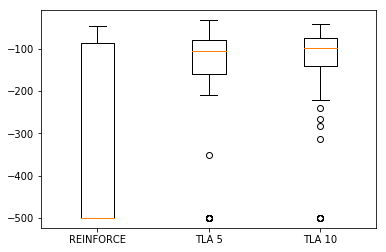
\includegraphics[width=.8\linewidth]{results/Acrobot/no_sparse_transfer/asymp_target_re-akt5-akt10.png}
    \caption{Asymptotic performances}
\end{figure}
\note{
    \begin{itemize}
        \item asymptotic performances gives more info here
        \item our algorithm is again better
        \item Asymp. performances for REINFORCE vary a lot\dots
        \item But most of the times we don't get past minimum reward
        \item No significant difference between TLA 5 \& TLA 10
    \end{itemize}
}
\end{frame}

\begin{frame}[fragile]{Transfer of sparse representation}
\framesubtitle{Cart-pole}
\vskip1.5cm plus 0.5cm minus 0.1cm
Also transfer a randomly chosen sparse representation.
\begin{center}
    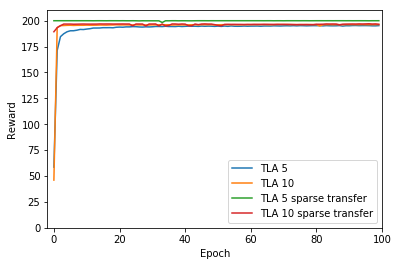
\includegraphics[width=.55\linewidth]{results/CartPole/sparse_transfer/reward_target_without_with.png}
\end{center}
    \begin{tabular}{llccc}
    \hline
    Algorithm & Sparse transfer & Mean & SD & Median \\
    \hline
       \textit{TLA 5} & No & $158.237$ & $23.153$ & $163.840$ \\
       \textit{TLA 10} & No & $165.120$ & $21.955$ & $169.034$ \\
       \textit{TLA 5} & Yes & $192.613$ & $28.179$ & $\bm{200.000}$ \\
       \textit{TLA 10} & Yes & $\bm{196.125}$ & $21.640$ & $\bm{200.000}$ \\
    \hline
    \end{tabular}
\note{
    \begin{itemize}
        \item Same asymptotic performances
        \item Median jumpstart for Sparse: $200$ instead of about $165$
    \end{itemize}
}
\end{frame}

\begin{frame}[fragile]{Transfer of sparse representation}
\framesubtitle{Acrobot}
\vskip0pt plus 3fill
\begin{center}
    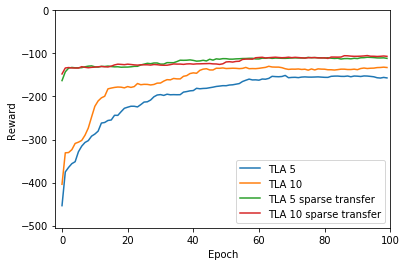
\includegraphics[width=.8\linewidth]{results/Acrobot/sparse_transfer/reward_target_without_with.png}
\end{center}
\note{
    \begin{itemize}
        \item Both jumpstart \& asymptotic performances are better
        \item No significant difference between TLA 5 sparse \& TLA 10 sparse
    \end{itemize}
}
\end{frame}

\begin{frame}[fragile]{REINFORCE using a source and target task}
\framesubtitle{Cart-pole}
\vskip1.5cm plus 0.5cm minus 0.1cm
Transfer of ANN weights.
\begin{center}
    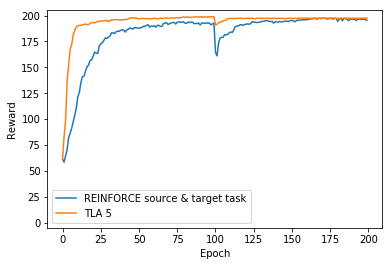
\includegraphics[width=.8\linewidth]{results/CartPole/reinforce_2tasks.png}
\end{center}
\note{
    \begin{itemize}
        \item REINFORCE first on source task then on target task
        \item Learns faster
        \item Higher jumpstart performance
        \item Same asymptotic performance
    \end{itemize}
}
\end{frame}

\begin{frame}[fragile]{REINFORCE using a source and target task}
\framesubtitle{Acrobot}
\vskip0pt plus 3fill
\begin{center}
    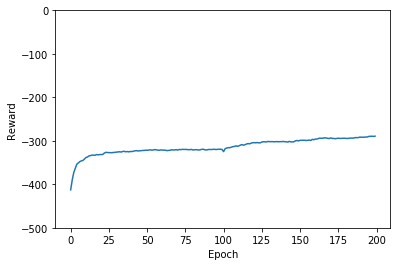
\includegraphics[width=.7\linewidth]{results/Acrobot/reinforce_2tasks.png}
\end{center}
\begin{tabular}{llccc}
\hline
Algorithm & Jumpstart & Asymptotic \\
\hline
   \textit{REINFORCE source \& target} & $-500$ & $-203.426$ \\
   \textit{TLA 5} & $\bm{-110.482}$ & $\bm{-93.085}$ \\
\hline
\end{tabular}
(medians)
\note{
    \begin{itemize}
        \item Learns faster
        \item Higher jumpstart performance
        \item Higher asymptotic performance
    \end{itemize}
}
\end{frame}

\part{Conclusions}
\section{Conclusions}
\begin{frame}[fragile]{Conclusions}
\begin{itemize}
    \item It's better to use transfer learning
    \begin{itemize}
        \item Our algorithm performs better than \textit{REINFORCE}
    \end{itemize}
    \item It is better to use multiple source tasks
    \item Parallel learning on source tasks better than sequentially
    \item Feature extraction wasn't beneficial for our environments
\end{itemize}
\note{
    \begin{itemize}
        \item It's better to use transfer learning
        \begin{itemize}
            \item Our algorithm performs better than \textit{REINFORCE}
        \end{itemize}
        \item It is better to use multiple source tasks
        \item Parallel learning on source tasks better than sequentially
        \item Feature extraction wasn't beneficial for our environments
    \end{itemize}
}
\end{frame}

\begin{frame}[fragile]{Conclusions}
\framesubtitle{Future work}
\begin{itemize}
    \item Apply on environments with feature extraction (e.g. \textit{Pong}, \textit{Breakout})
    \item Transfer between different environments
    \begin{itemize}
        \item Using task mappings
    \end{itemize}
\end{itemize}
\note{
    \begin{itemize}
        \item Apply on environments with feature extraction (e.g. \textit{Pong}, \textit{Breakout})
        \item For example using CNN
        \item Transfer between different environments
        \begin{itemize}
            \item Using task mappings
        \end{itemize}
    \end{itemize}
}
\end{frame}

\begin{frame}[c]{The end}
\begin{center}
    \color{vubbleu} \LARGE\vubfont Thank you for listening!
\end{center}
\end{frame}

\begin{frame}[allowframebreaks]
\frametitle{References}
\footnotesize{
\bibliographystyle{apalike}
\bibliography{../Mendeley.bib}
}
\end{frame}

\end{document}
